%%%%%%%%%%%%%%%%%%%%%%%%%%%%%%%%%%%%%%%%%
% Classicthesis Typographic Thesis
% LaTeX Template
% Version 1.0 (23/4/12)
%
% This template has been downloaded from:
% http://www.LaTeXTemplates.com
%
% Original author:
% Andr� Miede (http://www.miede.de)
%
% License:
% CC BY-NC-SA 3.0 (http://creativecommons.org/licenses/by-nc-sa/3.0/)
%
% General Tips:
% 1) Make sure to edit the classicthesis-config.file
% 2) New enumeration (A., B., C., etc in small caps): \begin{aenumerate} \end{aenumerate}
% 3) For margin notes: \marginpar or \graffito{}
% 4) Do not use bold fonts in this style, it is designed around them
% 5) Use tables as in the examples
% 6) See classicthesis-preamble.sty for useful commands
%
%%%%%%%%%%%%%%%%%%%%%%%%%%%%%%%%%%%%%%%%%

%----------------------------------------------------------------------------------------
%	PACKAGES AND OTHER DOCUMENT CONFIGURATIONS
%----------------------------------------------------------------------------------------

\documentclass[
		twoside,openright,titlepage,numbers=noenddot,headinclude,%1headlines,
                footinclude=true,cleardoublepage=empty,
                BCOR=5mm,paper=a4,fontsize=11pt, % Binding correction, paper type and font size
                ngerman,american, % Languages
                ]{scrreprt} 
                
% Includes the file which contains all the document configurations and packages - make sure to edit this file
%%%%%%%%%%%%%%%%%%%%%%%%%%%%%%%%%%%%%%%%%
% Thesis Configuration File
%
% The main lines to change in this file are in the DOCUMENT VARIABLES
% section, the rest of the file is for advanced configuration.
%
%%%%%%%%%%%%%%%%%%%%%%%%%%%%%%%%%%%%%%%%%

%----------------------------------------------------------------------------------------
%	DOCUMENT VARIABLES
%	Fill in the lines below to enter your information into the thesis template
%	Each of the commands can be cited anywhere in the thesis
%----------------------------------------------------------------------------------------

% Remove drafting to get rid of the '[ Date - classicthesis version 4.0 ]' text at the bottom of every page
\PassOptionsToPackage{eulerchapternumbers,listings,drafting, pdfspacing, subfig,beramono,eulermath,parts,dottedtoc}{classicthesis}
% Available options: drafting parts nochapters linedheaders eulerchapternumbers beramono eulermath pdfspacing minionprospacing tocaligned dottedtoc manychapters listings floatperchapter subfig
% Adding 'dottedtoc' will make page numbers in the table of contents flushed right with dots leading to them

\newcommand{\myTitle}{GIRAF Launcher\xspace}
\newcommand{\mySubtitle}{An Homage to The Elements of Typographic Style\xspace}
\newcommand{\myDegree}{Doktor-Ingenieur (Dr.-Ing.)\xspace}
\newcommand{\myName}{Andr\'e Miede\xspace}
\newcommand{\myProf}{Put name here\xspace}
\newcommand{\myOtherProf}{Put name here\xspace}
\newcommand{\mySupervisor}{Put name here\xspace}
\newcommand{\myFaculty}{Put data here\xspace}
\newcommand{\myDepartment}{Put data here\xspace}
\newcommand{\myUni}{Put data here\xspace}
\newcommand{\myLocation}{Darmstadt\xspace}
\newcommand{\myTime}{December 2011\xspace}
\newcommand{\myVersion}{version 4.0\xspace}

%----------------------------------------------------------------------------------------
%	USEFUL COMMANDS
%----------------------------------------------------------------------------------------

\newcommand{\ie}{i.\,e.}
\newcommand{\Ie}{I.\,e.}
\newcommand{\eg}{e.\,g.}
\newcommand{\Eg}{E.\,g.} 

\newcounter{dummy} % Necessary for correct hyperlinks (to index, bib, etc.)
\providecommand{\mLyX}{L\kern-.1667em\lower.25em\hbox{Y}\kern-.125emX\@}

%----------------------------------------------------------------------------------------
%	PACKAGES
%----------------------------------------------------------------------------------------

\usepackage{lipsum} % Used for inserting dummy 'Lorem ipsum' text into the template

%------------------------------------------------
 
\PassOptionsToPackage{latin9}{inputenc} % latin9 (ISO-8859-9) = latin1+"Euro sign"
\usepackage{inputenc}
 
 %------------------------------------------------

%\PassOptionsToPackage{ngerman,american}{babel}  % Change this to your language(s)
% Spanish languages need extra options in order to work with this template
%\PassOptionsToPackage{spanish,es-lcroman}{babel}
\usepackage{babel}

%------------------------------------------------			

\PassOptionsToPackage{square,numbers}{natbib}
 \usepackage{natbib}
 
 %------------------------------------------------

\PassOptionsToPackage{fleqn}{amsmath} % Math environments and more by the AMS 
 \usepackage{amsmath}
 
 %------------------------------------------------

\PassOptionsToPackage{T1}{fontenc} % T2A for cyrillics
\usepackage{fontenc}

%------------------------------------------------

\usepackage{xspace} % To get the spacing after macros right

%------------------------------------------------

\usepackage{mparhack} % To get marginpar right

%------------------------------------------------

\usepackage{fixltx2e} % Fixes some LaTeX stuff 

%------------------------------------------------

\PassOptionsToPackage{smaller}{acronym} % Include printonlyused in the first bracket to only show acronyms used in the text
\usepackage{acronym} % nice macros for handling all acronyms in the thesis

%------------------------------------------------

%\renewcommand*{\acsfont}[1]{\textssc{#1}} % For MinionPro
\renewcommand{\bflabel}[1]{{#1}\hfill} % Fix the list of acronyms

%------------------------------------------------

\PassOptionsToPackage{pdftex}{graphicx}
\usepackage{graphicx} 

%----------------------------------------------------------------------------------------
%	FLOATS: TABLES, FIGURES AND CAPTIONS SETUP
%----------------------------------------------------------------------------------------

\usepackage{tabularx} % Better tables
\setlength{\extrarowheight}{3pt} % Increase table row height
\newcommand{\tableheadline}[1]{\multicolumn{1}{c}{\spacedlowsmallcaps{#1}}}
\newcommand{\myfloatalign}{\centering} % To be used with each float for alignment
\usepackage{caption}
\captionsetup{format=hang,font=small}
\usepackage{subfig}  

%----------------------------------------------------------------------------------------
%	CODE LISTINGS SETUP
%----------------------------------------------------------------------------------------

\usepackage{listings} 
\usepackage{color} %For sourceCode listnings

%\lstset{emph={trueIndex,root},emphstyle=\color{BlueViolet}}%\underbar} % for special keywords
\lstset{language=[LaTeX]Tex, % Specify the language for listings here
keywordstyle=\color{RoyalBlue}, % Add \bfseries for bold
basicstyle=\small\ttfamily, % Makes listings a smaller font size and a different font
%identifierstyle=\color{NavyBlue}, % Color of text inside brackets
commentstyle=\color{Green}\ttfamily, % Color of comments
stringstyle=\rmfamily, % Font type to use for strings
numbers=left, % Change left to none to remove line numbers
numberstyle=\scriptsize, % Font size of the line numbers
stepnumber=5, % Increment of line numbers
numbersep=8pt, % Distance of line numbers from code listing
showstringspaces=false, % Sets whether spaces in strings should appear underlined
breaklines=true, % Force the code to stay in the confines of the listing box
%frameround=ftff, % Uncomment for rounded frame
frame=single, % Frame border - none/leftline/topline/bottomline/lines/single/shadowbox/L
belowcaptionskip=.75\baselineskip % Space after the "Listing #: Desciption" text and the listing box
}


%%%%%%%%%%%%%%%%%%%%%%%%
%% Steiniche was here %%
%%%%%%%%%%%%%%%%%%%%%%%%
\definecolor{gray95}{gray}{.95}
\lstdefinestyle{sourceCode}
{ 
 numbers=left,
 numbersep=5pt, 
 stepnumber=1,
 captionpos=b,  %bottom
 keywordstyle=\color{purple},
 commentstyle=\color[rgb]{0.133,0.545,0.133},
 stringstyle=\color[rgb]{0.627,0.126,0.941},
 backgroundcolor=\color{gray95},
 frame=lrtb,
 framerule=0.5pt,
 linewidth=\textwidth,
 tabsize=4,
 numberbychapter=true,
 basicstyle=\ttfamily\footnotesize,
 language=[Sharp]C,
 breaklines=true,
 showstringspaces=false,
 emph=[2]{Tag,Problem,Person,List,NotSupportedException,TestMethod,ProblemSearch,Assert,
 EntityCollection,Department,IEnumerable,TimeSpan,DateTime},%%Classes
 emphstyle=[2]{\color[rgb]{0.1,0.5,0.5}},
 float=htb,
 breakindent=20pt
}



%----------------------------------------------------------------------------------------
%	Quoteations
%----------------------------------------------------------------------------------------
\newcolumntype{R}{>{\raggedleft\arraybackslash}X}%

\def\changemargin#1#2{\list{}{\rightmargin#2\leftmargin#1}\item[]}
\let\endchangemargin=\endlist
\newcommand{\myQuoteA}[2]{
\begin{changemargin}{.7in}{.7in}
\textbf{``}
#1
\textbf{''}
\ifthenelse{\isempty{#2}}%  If there is nothing stated here just print the shit. 
{}% if #1 true
{\vspace{-3mm}\begin{changemargin}{.9in}{.7in}\raggedleft{{\footnotesize--- #2}}\end{changemargin}}% if #1 false
\end{changemargin}
}

\newcommand{\myQuote}[1]{\myQuoteA{#1}{}}

%----------------------------------------------------------------------------------------
%	HYPERREFERENCES
%----------------------------------------------------------------------------------------

\PassOptionsToPackage{pdftex,hyperfootnotes=false,pdfpagelabels}{hyperref}
\usepackage{hyperref}  % backref linktocpage pagebackref
\pdfcompresslevel=9
\pdfadjustspacing=1

\hypersetup{
% Uncomment the line below to remove all links (to references, figures, tables, etc)
%draft, 
colorlinks=true, linktocpage=true, pdfstartpage=3, pdfstartview=FitV,
% Uncomment the line below if you want to have black links (e.g. for printing black and white)
%colorlinks=false, linktocpage=false, pdfborder={0 0 0}, pdfstartpage=3, pdfstartview=FitV, 
breaklinks=true, pdfpagemode=UseNone, pageanchor=true, pdfpagemode=UseOutlines,
plainpages=false, bookmarksnumbered, bookmarksopen=true, bookmarksopenlevel=1,
hypertexnames=true, pdfhighlight=/O, urlcolor=webbrown, linkcolor=RoyalBlue, citecolor=webgreen,
%------------------------------------------------
% PDF file meta-information
pdftitle={\myTitle},
pdfauthor={\textcopyright\ \myName, \myUni, \myFaculty},
pdfsubject={},
pdfkeywords={},
pdfcreator={pdfLaTeX},
pdfproducer={LaTeX with hyperref and classicthesis}
%------------------------------------------------
}   

%----------------------------------------------------------------------------------------
%	BACKREFERENCES
%----------------------------------------------------------------------------------------

\usepackage{ifthen} % Allows the user of the \ifthenelse command
\newboolean{enable-backrefs} % Variable to enable backrefs in the bibliography
\setboolean{enable-backrefs}{false} % Variable value: true or false

\newcommand{\backrefnotcitedstring}{\relax} % (Not cited.)
\newcommand{\backrefcitedsinglestring}[1]{(Cited on page~#1.)}
\newcommand{\backrefcitedmultistring}[1]{(Cited on pages~#1.)}
\ifthenelse{\boolean{enable-backrefs}} % If backrefs were enabled
{
\PassOptionsToPackage{hyperpageref}{backref}
\usepackage{backref} % to be loaded after hyperref package 
\renewcommand{\backreftwosep}{ and~} % separate 2 pages
\renewcommand{\backreflastsep}{, and~} % separate last of longer list
\renewcommand*{\backref}[1]{}  % disable standard
\renewcommand*{\backrefalt}[4]{% detailed backref
\ifcase #1 
\backrefnotcitedstring
\or
\backrefcitedsinglestring{#2}
\else
\backrefcitedmultistring{#2}
\fi}
}{\relax} 

%----------------------------------------------------------------------------------------
%	AUTOREFERENCES SETUP
%	Redefines how references in text are prefaced for different 
%	languages (e.g. "Section 1.2" or "section 1.2")
%----------------------------------------------------------------------------------------

\makeatletter
\@ifpackageloaded{babel}
{
\addto\extrasamerican{
\renewcommand*{\figureautorefname}{Figure}
\renewcommand*{\tableautorefname}{Table}
\renewcommand*{\partautorefname}{Part}
\renewcommand*{\chapterautorefname}{Chapter}
\renewcommand*{\sectionautorefname}{Section}
\renewcommand*{\subsectionautorefname}{Section}
\renewcommand*{\subsubsectionautorefname}{Section}
}
\addto\extrasngerman{
\renewcommand*{\paragraphautorefname}{Absatz}
\renewcommand*{\subparagraphautorefname}{Unterabsatz}
\renewcommand*{\footnoteautorefname}{Fu\"snote}
\renewcommand*{\FancyVerbLineautorefname}{Zeile}
\renewcommand*{\theoremautorefname}{Theorem}
\renewcommand*{\appendixautorefname}{Anhang}
\renewcommand*{\equationautorefname}{Gleichung}
\renewcommand*{\itemautorefname}{Punkt}
}
\providecommand{\subfigureautorefname}{\figureautorefname} % Fix to getting autorefs for subfigures right
}{\relax}
\makeatother

%----------------------------------------------------------------------------------------

\usepackage{classicthesis} 

%----------------------------------------------------------------------------------------
%	CHANGING TEXT AREA 
%----------------------------------------------------------------------------------------

%\linespread{1.05} % a bit more for Palatino
%\areaset[current]{312pt}{761pt} % 686 (factor 2.2) + 33 head + 42 head \the\footskip
%\setlength{\marginparwidth}{7em}%
%\setlength{\marginparsep}{2em}%

%----------------------------------------------------------------------------------------
%	USING DIFFERENT FONTS
%----------------------------------------------------------------------------------------

%\usepackage[oldstylenums]{kpfonts} % oldstyle notextcomp
%\usepackage[osf]{libertine}
%\usepackage{hfoldsty} % Computer Modern with osf
%\usepackage[light,condensed,math]{iwona}
%\renewcommand{\sfdefault}{iwona}
%\usepackage{lmodern} % <-- no osf support :-(
%\usepackage[urw-garamond]{mathdesign} <-- no osf support :-(


% to get lastpage
%\usepackage{lastpage}

\usepackage{verbatim}
\usepackage{casecontrol}
\usepackage{ifthen}
\usepackage{xifthen}

% fixme's
%\usepackage{xkvltxp}
\usepackage[footnote,draft,english,silent,nomargin]{fixme}
\newcommand{\todo}[1]{\fxnote{#1}}
\newcommand{\localgroup}[1][]{\caseControl{p}{roject group}{#1}{}}
\newcommand{\globalgroup}[1][]{\caseControl{m}{ultiproject group}{#1}{}}
\newcommand{\egebakken}[1][]{{Egebakken}{#1}{}}
\newcommand{\guardian}[1][]{\caseControl{g}{uardian}{#1}{}}
\newcommand{\autist}[1][]{\caseControl{c}{hild with austim}{#1}{}}
\newcommand{\autists}[1][]{\caseControl{c}{hildren with austim}{#1}{}}
\newcommand{\giraf}[1][]{{GIRAF}{#1}{}}
\newcommand{\guicomponents}[1][]{{\giraf[] GUI Components}{#1}{}}
\newcommand{\girafapp}[1][]{{\giraf[] app}{#1}{}}

\newcommand{\method}[1]{\emph{#1}}
\newcommand{\class}[1]{\emph{#1}}
\newcommand{\activity}[1]{\emph{#1}}

% to get \newevenside :
\usepackage{ifthen}
\newcommand{\newevenside}{
        \ifthenelse{\isodd{\thepage}}{\newpage}{
        \newpage
        \phantom{placeholder} % doesn't appear on page
        \thispagestyle{empty} % if want no header/footer
        \newpage
        }
}

\begin{document}

\frenchspacing % Reduces space after periods to make text more compact

\raggedbottom % Makes all pages the height of the text on that page

\selectlanguage{american} % Select your default language - e.g. american or ngerman

%\renewcommand*{\bibname}{new name} % Uncomment to change the name of the bibliography
%\setbibpreamble{} % Uncomment to include a preamble to the bibliography - some text before the reference list starts

\pagenumbering{roman} % Roman page numbering prior to the start of the thesis content (i, ii, iii, etc)

\pagestyle{plain} % Suppress headers for the pre-content pages

%----------------------------------------------------------------------------------------
%	PRE-CONTENT THESIS PAGES
%----------------------------------------------------------------------------------------

%% Title Page

\begin{titlepage}
%
\includepdf[pages=-]{gfx/frontpage.pdf}



\includegraphics[width=\textwidth,height=\textheight]{gfx/frontpage.pdf}



% \begin{addmargin}[-1cm]{-3cm}
% \begin{center}
% \large
% 
% \hfill
% \vfill
% 
% \begingroup
% \color{Maroon}\spacedallcaps{\myTitle} \\ \bigskip % Thesis title
% \endgroup
% 
% \spacedlowsmallcaps{\myName} % Your name
% 
% \vfill
% 
% 
\includegraphics[width=6cm]{gfx/TFZsuperellipse_bw} \\ \medskip % Picture
% 
% \mySubtitle \\ \medskip % Thesis subtitle
% %\myDegree \\
% %\myDepartment \\
% %\myFaculty \\
% %\myUni \\ \bigskip
% 
% \myTime\ -- \myVersion % Time and version
% 
% \vfill
% 
% \end{center}
% \end{addmargin}

\end{titlepage} % Main title page

%% Back of the title page

\thispagestyle{empty}

\hfill

\vfill

\noindent\myName: \textit{\myTitle,} \mySubtitle, %\myDegree, 
\textcopyright\ \myTime

% You may wish to do something with the back of the title page, such as including your supervisors, location or time frame of the work. Below is an example of doing so although you may want to tweak it to your liking.

%\bigskip

%\noindent\spacedlowsmallcaps{Supervisors}: \\
%\myProf \\
%\myOtherProf \\ 
%\mySupervisor

%\medskip \\

%\noindent\spacedlowsmallcaps{Location}: \\
%\myLocation

%\medskip \\

%\noindent\spacedlowsmallcaps{Time Frame}: \\
%\myTime
 % Back of the title page

%\cleardoublepage% Abstract

\pdfbookmark[1]{Abstract}{Abstract} % Bookmark name visible in a PDF viewer

\begingroup
\let\clearpage\relax
\let\cleardoublepage\relax
\let\cleardoublepage\relax

\chapter*{Abstract} % Abstract name

Short summary of the contents\dots

\endgroup			

\vfill % Abstract page

%\cleardoublepage% Publications - a page listing research articles written using content in the thesis

\pdfbookmark[1]{Publications}{Publications} % Bookmark name visible in a PDF viewer

\chapter*{Publications} % Publications page text

Some ideas and figures have appeared previously in the following publications:

\bigskip

\noindent Put your publications from the thesis here. The packages \texttt{multibib} or \texttt{bibtopic} etc. can be used to handle multiple different bibliographies in your document. % Publications from the thesis page

%\cleardoublepage\pdfbookmark[1]{Acknowledgements}{Acknowledgements} % Bookmark name visible in a PDF viewer

% \begin{flushright}{\slshape    
% We have seen that computer programming is an art, \\ 
% because it applies accumulated knowledge to the world, \\ 
% because it requires skill and ingenuity, and especially \\
% because it produces objects of beauty.} \\ \medskip
% --- \defcitealias{knuth:1974}{Donald E. Knuth}\citetalias{knuth:1974} \citep{knuth:1974}
% \end{flushright}
% 
% \bigskip
% 
% %----------------------------------------------------------------------------------------

\begingroup

\let\clearpage\relax
\let\cleardoublepage\relax
\let\cleardoublepage\relax

\chapter*{Acknowledgements}

\noindent We would like to thank our supervisor, Ulrik Mathias Nyman, for both the extensive and professional guidance as well as motivation. We would also like to thank \emph{Naked Fruit} \citep{web:nakedfruit} for supplying refreshing drinks. Thanks to Henrik S\o{}rensen, Peter Axel Nielsen, Ivan Aaen, and Michael Skov, for advice during the design process.

\noindent As a multiproject group, we wish to acknowledge the help and time spent by the educators and teachers from various institutions, whose insight has been of utmost value in the development of the \giraf[] system.

% \noindent Regarding the typography and other help, many thanks go to Marco Kuhlmann, Philipp Lehman, Lothar Schlesier, Jim Young, Lorenzo Pantieri and Enrico Gregorio\footnote{Members of GuIT (Gruppo Italiano Utilizzatori di \TeX\ e \LaTeX )}, J\"org Sommer, Joachim K\"ostler, Daniel Gottschlag, Denis Aydin, Paride Legovini, Steffen Prochnow, Nicolas Repp, Hinrich Harms, Roland Winkler,  and the whole \LaTeX-community for support, ideas and some great software.
% 
% \bigskip
% 
% \noindent\emph{Regarding \mLyX}: The \mLyX\ port was intially done by
% \emph{Nicholas Mariette} in March 2009 and continued by
% \emph{Ivo Pletikosi\'c} in 2011. Thank you very much for your work and the contributions to the original style.

\endgroup % Acknowledgements page


\listoffixmes
\newpage

\pagestyle{scrheadings} % Show chapter titles as headings





\section{External Architecture}

\autoref{fig:external_architecture} illustrates the \giraf[] launcher component. The component provides one service and have one dependency. The services it provides is based on demands from the surrounding components of the \giraf[] platform, which can be seen in \autoref{cmn:fig:architecture}. The illustrated service provides a way for launched \girafapp[]s to determine which guardian launched the application in question, and with which child profile. The illustrated dependency represents the need for being able to read and update profile data. The service which fulfill this dependency is provided by Oasis. 

As seen on \autoref{cmn:fig:architecture}, Oasis is available for the launcher to use. This database stores the modulated data, including the guardian and child profiles.


\begin{figure}[h]
	\centering
	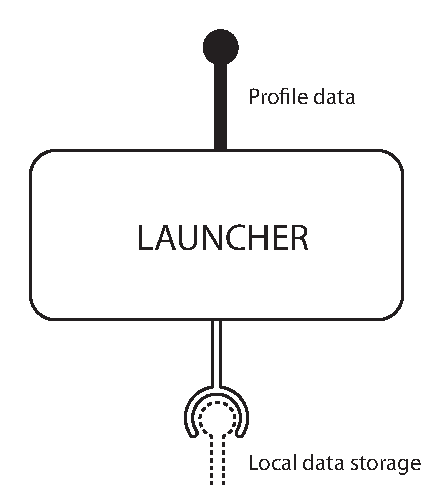
\includegraphics[width=0.5\textwidth]{gfx/external_launcher_architecture.pdf}
	\caption{The external architecture of the \giraf[] launcher.}
	\label{fig:external_architecture}
\end{figure}

%%%%%%%%%%%%%%%%%%%%%%%%%%%%%%%%%%%%%%%%%%%%%%%%%%%%%%%%%%%%%%%%%%%%%%%%%%%%%%%%%%%% COMMENT
\begin{comment}
Two external architectures are described in this section, namely those of the \giraf[] launcher, and the \guicomponents[] library.

\subsection{\giraf[] Launcher}
\label{sec:launcher_architecture}
The external architecture of the launcher can be seen in \autoref{fig:external_architecture}.
\begin{figure}[h]
	\centering
	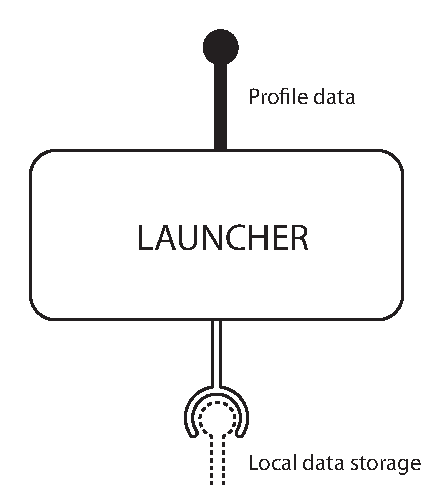
\includegraphics[width=0.5\textwidth]{gfx/external_launcher_architecture.pdf}
	\caption{The external architecture of the \giraf[] launcher.}
	\label{fig:external_architecture}
\end{figure}
The launcher provides two essential services: The ability for users to run, i.e. \textit{launch}, apps, and the provisioning of profile data to these apps. 
The launcher currently allows only \giraf[] apps to be used, but this is by design, as the launcher currently does not support addition and removal of apps. 
The profile data service allows a \guardian[] profile to select a child profile to use a given app with. 
Both the ID of the \guardian[] profile and the child profile is then provided to the app, in order to make it easy for a \guardian[] to switch between different children as needed, while maintaining specific app customizations for different profiles. \newline

The \giraf[] launcher has only one dependancy in the \giraf[] system, namely the Oasis database. 
The launcher is heavily integrated with Oasis, and as such requires the Oasis database to be installed on the device to function. 
Services utilized by the launcher include profile authentication, saving and loading of settings and app integration. 

\subsection{\guicomponents[]}
The \guicomponents[] architecture is designed to be flexible. 
The flexibility is important to keep the \guicomponents[] open and changeable by anyone involved in the development of \giraf[]. 
As such, the only architectural requirement for components that are added to \guicomponents[], is that they should be based on existing Android UI components. 
The philosophy behind this architecture, is that by using existing Android UI components, with a new layout and possible added functionality, the components are already well defined and fully supported in Android. 
The example shown in \autoref{fig:gui_comp_architecture} highlights a possible way of incorporating a component, assuming the need for a customized button: \textit{GButton}. 
\begin{figure}[h]
	\centering
	
\includegraphics[width=1\textwidth]{gfx/gui_components_architecture.pdf}
	\caption{\guicomponents[] Architecture Example}
	\label{fig:gui_comp_architecture}
\end{figure}
\end{comment}
\section{Internal Architecture}

Being able to launch an \girafapp[] as a specific guardian requires that the user interacts such that the launcher knows which guardian the user represents.

Authentication is chosen, as each modulated child and guardian contains private data. QR-codes are chosen as means of authentication, as they provide a level of security.

An alternative to QR-codes could be a \emph{username-password} method, where each user have their own username, with an private password. The system is designed to have the two modes: guardian- and child mode\todo{ref til backlog}. A username-password combination requires the user to remember their credentials, whereas some \autists[] have problems with it. \todo{quote drazenko - vent paa mail fra accept}

%\myquote{Some children with autism can have a hard time remembering a username and a password}
 - Drazenko Banjak, english translation. Native language quote can be seen in \autoref{FIXME}\todo{indsaet i appendix "Nogle børn med autisme kan have svært ved at skulle huske et brugernavn og en adgangskode."}

QR codes provides a physical way of storing the user credentials and allows for other users to take responsibility of the QR-code, such as a \guardian[] carrying a QR-code of a \autist[].

QR-codes can be scanned by a built-in camera on tablets and can be printed using standard paper and printer equipment. 

QR-codes are copyable, by e.g. a copymachine, and therefore must be kept away from untrusted users, if they should not be used by people for which they were not intended.

To sum up, QR-codes are chosen because of they improve usability, despite of their ability to be copied.\todo{Ulrik, er dette i orden?}


%%%%%%%%%%%%%%%%%%%%%%%%%%%%%%%%%%%%%%%%%%%%%% COMMENT
\begin{comment}
\begin{figure}[h]
	\centering
	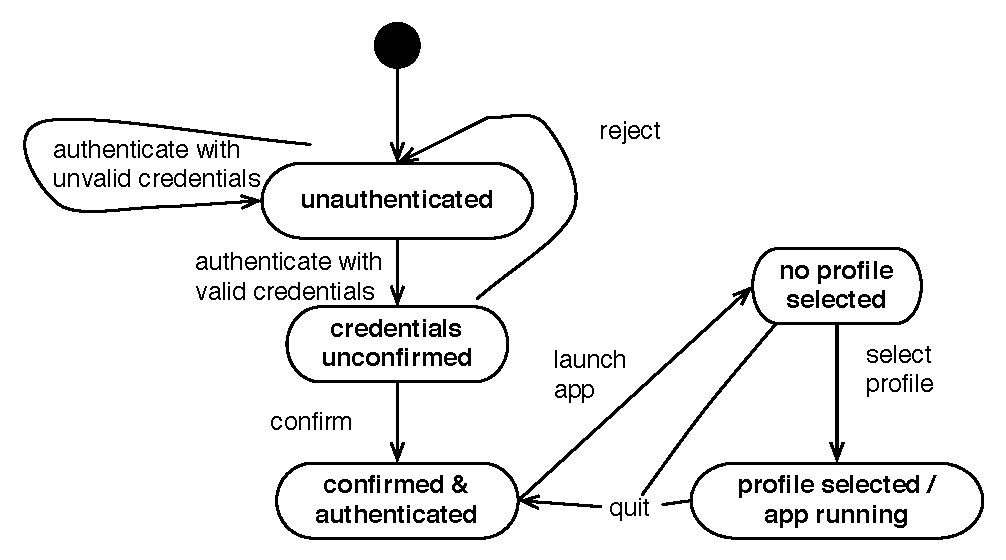
\includegraphics[width=1\textwidth]{gfx/flow-diagram2.pdf}
	\caption{Flow diagram}
	\label{fig:flow_diagram}
\end{figure}

\autoref{fig:flow_diagram} shows the state of the launcher. The first three states handles the distinction between users which are allowed to access the launchable applications, and those who are not. \todo{indsaet ref til der hvor vi fandt ud af at vi skulle have authentication}

Based on \autoref{fig:flow_diagram}, ..
\end{comment}







%\cleardoublepage
\cleardoublepage
% Table of Contents - List of Tables/Figures/Listings and Acronyms

\refstepcounter{dummy}

\pdfbookmark[1]{\contentsname}{tableofcontents} % Bookmark name visible in a PDF viewer

\setcounter{tocdepth}{2} % Depth of sections to include in the table of contents - currently up to subsections

\setcounter{secnumdepth}{3} % Depth of sections to number in the text itself - currently up to subsubsections

\manualmark
\markboth{\spacedlowsmallcaps{\contentsname}}{\spacedlowsmallcaps{\contentsname}}

\tableofcontents 

\automark[section]{chapter}
\renewcommand{\chaptermark}[1]{\markboth{\spacedlowsmallcaps{#1}}{\spacedlowsmallcaps{#1}}}
\renewcommand{\sectionmark}[1]{\markright{\thesection\enspace\spacedlowsmallcaps{#1}}}

\clearpage

\begingroup 
\let\clearpage\relax
\let\cleardoublepage\relax
\let\cleardoublepage\relax

%----------------------------------------------------------------------------------------
%	List of Figures
%----------------------------------------------------------------------------------------

\refstepcounter{dummy}
%\addcontentsline{toc}{chapter}{\listfigurename} % Uncomment if you would like the list of figures to appear in the table of contents
\pdfbookmark[1]{\listfigurename}{lof} % Bookmark name visible in a PDF viewer

\listoffigures

\vspace*{8ex}
\newpage

%----------------------------------------------------------------------------------------
%	List of Tables
%----------------------------------------------------------------------------------------

\refstepcounter{dummy}
%\addcontentsline{toc}{chapter}{\listtablename} % Uncomment if you would like the list of tables to appear in the table of contents
\pdfbookmark[1]{\listtablename}{lot} % Bookmark name visible in a PDF viewer

\listoftables
        
\vspace*{8ex}
\newpage
    
%----------------------------------------------------------------------------------------
%	List of Listings
%---------------------------------------------------------------------------------------- 

\refstepcounter{dummy}
%\addcontentsline{toc}{chapter}{\lstlistlistingname} % Uncomment if you would like the list of listings to appear in the table of contents
\pdfbookmark[1]{\lstlistlistingname}{lol} % Bookmark name visible in a PDF viewer

\lstlistoflistings 

\vspace*{8ex}
\newpage
       
%----------------------------------------------------------------------------------------
%	Acronyms
%----------------------------------------------------------------------------------------

\refstepcounter{dummy}
%\addcontentsline{toc}{chapter}{Acronyms} % Uncomment if you would like the acronyms to appear in the table of contents
\pdfbookmark[1]{Acronyms}{acronyms} % Bookmark name visible in a PDF viewer

\markboth{\spacedlowsmallcaps{Acronyms}}{\spacedlowsmallcaps{Acronyms}}

\chapter*{Acronyms}

\begin{acronym}[UML]
%\acro{DRY}{Don't Repeat Yourself}
\end{acronym}  
                   
\endgroup

\cleardoublepage % Contents, list of figures/tables/listings and acronyms

\pagenumbering{arabic} % Arabic page numbering for thesis content (1, 2, 3, etc)
%\setcounter{page}{90} % Uncomment to manually start the page counter at an arbitrary value (for example if you wish to count the pre-content pages in the page count)

\cleardoublepage % Avoids problems with pdfbookmark

%----------------------------------------------------------------------------------------
%	INTRODUCTION
%----------------------------------------------------------------------------------------



\section{External Architecture}

\autoref{fig:external_architecture} illustrates the \giraf[] launcher component. The component provides one service and have one dependency. The services it provides is based on demands from the surrounding components of the \giraf[] platform, which can be seen in \autoref{cmn:fig:architecture}. The illustrated service provides a way for launched \girafapp[]s to determine which guardian launched the application in question, and with which child profile. The illustrated dependency represents the need for being able to read and update profile data. The service which fulfill this dependency is provided by Oasis. 

As seen on \autoref{cmn:fig:architecture}, Oasis is available for the launcher to use. This database stores the modulated data, including the guardian and child profiles.


\begin{figure}[h]
	\centering
	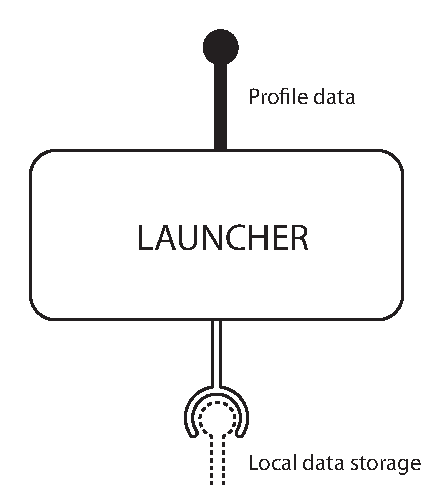
\includegraphics[width=0.5\textwidth]{gfx/external_launcher_architecture.pdf}
	\caption{The external architecture of the \giraf[] launcher.}
	\label{fig:external_architecture}
\end{figure}

%%%%%%%%%%%%%%%%%%%%%%%%%%%%%%%%%%%%%%%%%%%%%%%%%%%%%%%%%%%%%%%%%%%%%%%%%%%%%%%%%%%% COMMENT
\begin{comment}
Two external architectures are described in this section, namely those of the \giraf[] launcher, and the \guicomponents[] library.

\subsection{\giraf[] Launcher}
\label{sec:launcher_architecture}
The external architecture of the launcher can be seen in \autoref{fig:external_architecture}.
\begin{figure}[h]
	\centering
	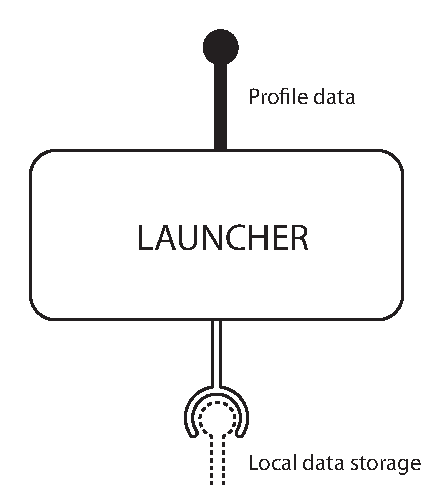
\includegraphics[width=0.5\textwidth]{gfx/external_launcher_architecture.pdf}
	\caption{The external architecture of the \giraf[] launcher.}
	\label{fig:external_architecture}
\end{figure}
The launcher provides two essential services: The ability for users to run, i.e. \textit{launch}, apps, and the provisioning of profile data to these apps. 
The launcher currently allows only \giraf[] apps to be used, but this is by design, as the launcher currently does not support addition and removal of apps. 
The profile data service allows a \guardian[] profile to select a child profile to use a given app with. 
Both the ID of the \guardian[] profile and the child profile is then provided to the app, in order to make it easy for a \guardian[] to switch between different children as needed, while maintaining specific app customizations for different profiles. \newline

The \giraf[] launcher has only one dependancy in the \giraf[] system, namely the Oasis database. 
The launcher is heavily integrated with Oasis, and as such requires the Oasis database to be installed on the device to function. 
Services utilized by the launcher include profile authentication, saving and loading of settings and app integration. 

\subsection{\guicomponents[]}
The \guicomponents[] architecture is designed to be flexible. 
The flexibility is important to keep the \guicomponents[] open and changeable by anyone involved in the development of \giraf[]. 
As such, the only architectural requirement for components that are added to \guicomponents[], is that they should be based on existing Android UI components. 
The philosophy behind this architecture, is that by using existing Android UI components, with a new layout and possible added functionality, the components are already well defined and fully supported in Android. 
The example shown in \autoref{fig:gui_comp_architecture} highlights a possible way of incorporating a component, assuming the need for a customized button: \textit{GButton}. 
\begin{figure}[h]
	\centering
	
\includegraphics[width=1\textwidth]{gfx/gui_components_architecture.pdf}
	\caption{\guicomponents[] Architecture Example}
	\label{fig:gui_comp_architecture}
\end{figure}
\end{comment}
\section{Internal Architecture}

Being able to launch an \girafapp[] as a specific guardian requires that the user interacts such that the launcher knows which guardian the user represents.

Authentication is chosen, as each modulated child and guardian contains private data. QR-codes are chosen as means of authentication, as they provide a level of security.

An alternative to QR-codes could be a \emph{username-password} method, where each user have their own username, with an private password. The system is designed to have the two modes: guardian- and child mode\todo{ref til backlog}. A username-password combination requires the user to remember their credentials, whereas some \autists[] have problems with it. \todo{quote drazenko - vent paa mail fra accept}

%\myquote{Some children with autism can have a hard time remembering a username and a password}
 - Drazenko Banjak, english translation. Native language quote can be seen in \autoref{FIXME}\todo{indsaet i appendix "Nogle børn med autisme kan have svært ved at skulle huske et brugernavn og en adgangskode."}

QR codes provides a physical way of storing the user credentials and allows for other users to take responsibility of the QR-code, such as a \guardian[] carrying a QR-code of a \autist[].

QR-codes can be scanned by a built-in camera on tablets and can be printed using standard paper and printer equipment. 

QR-codes are copyable, by e.g. a copymachine, and therefore must be kept away from untrusted users, if they should not be used by people for which they were not intended.

To sum up, QR-codes are chosen because of they improve usability, despite of their ability to be copied.\todo{Ulrik, er dette i orden?}


%%%%%%%%%%%%%%%%%%%%%%%%%%%%%%%%%%%%%%%%%%%%%% COMMENT
\begin{comment}
\begin{figure}[h]
	\centering
	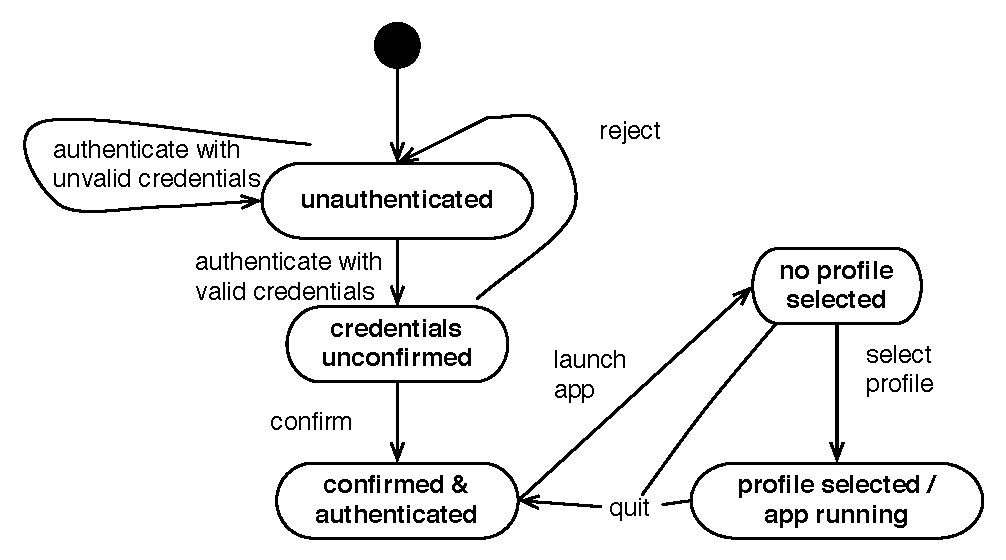
\includegraphics[width=1\textwidth]{gfx/flow-diagram2.pdf}
	\caption{Flow diagram}
	\label{fig:flow_diagram}
\end{figure}

\autoref{fig:flow_diagram} shows the state of the launcher. The first three states handles the distinction between users which are allowed to access the launchable applications, and those who are not. \todo{indsaet ref til der hvor vi fandt ud af at vi skulle have authentication}

Based on \autoref{fig:flow_diagram}, ..
\end{comment}



%----------------------------------------------------------------------------------------
%	POST-CONTENT
%----------------------------------------------------------------------------------------
\cleardoublepage\appendix
\chapter{Implementation}
\section{Logo Activity}
\begin{figure}[h!]
	\centering
	
\includegraphics[scale=0.3]{gfx/logo-activity_1.jpg}
	\caption{Portrait Logo Activity only shown when user do not have a valid session.}
	\label{fig:logo-activity_1}
\end{figure}
\begin{figure}[h!]
	\centering
	
\includegraphics[scale=0.3]{gfx/logo-activity_2.jpg}
	\caption{Landscape Logo Activity only shown when user has an valid session in and start the application again.}
	\label{fig:logo-activity_2}
\end{figure}
\section{Profile select activity}
\begin{figure}[h!]
	\centering
	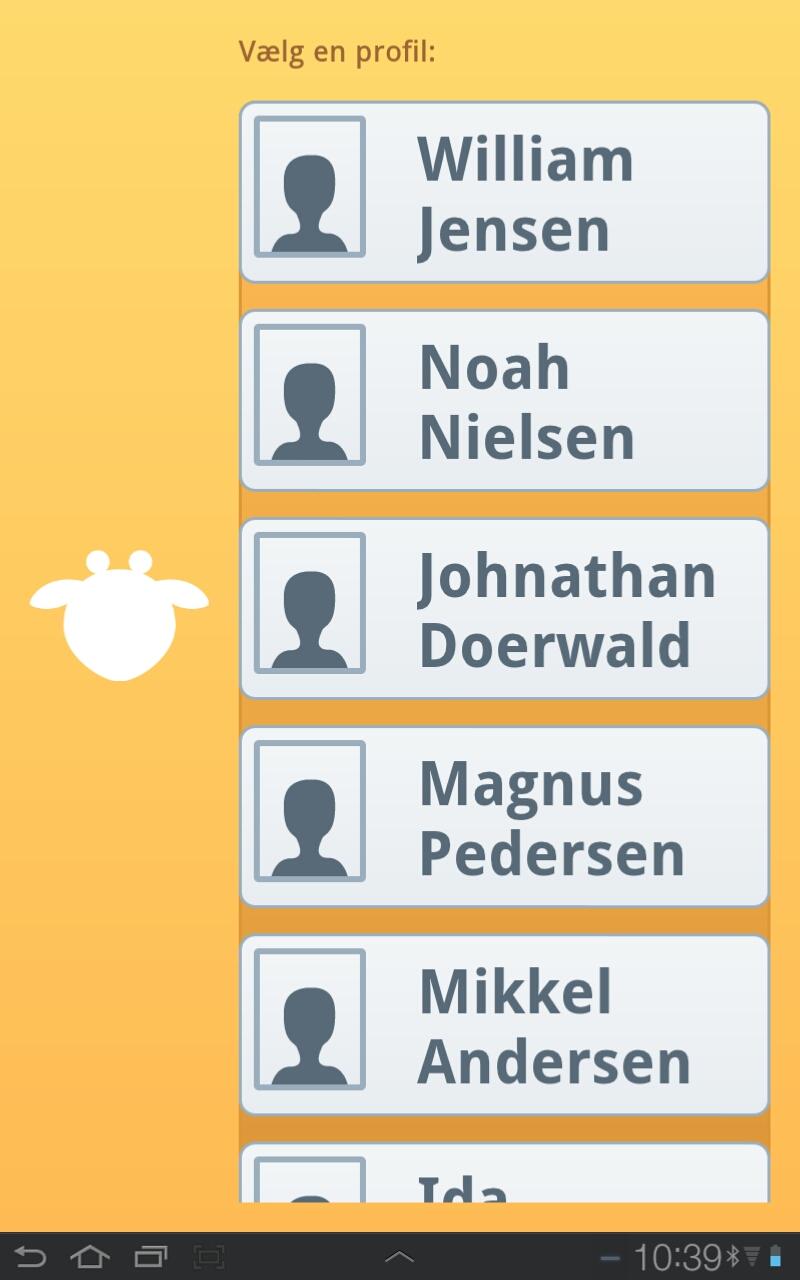
\includegraphics[scale=0.3]{gfx/profile-select-activity_1.jpg}
	\caption{Portrait profile select activity screenshot}
	\label{fig:profile-select-activity_1}
\end{figure}

\chapter{Use Cases}
\label{appendix_use_cases}

\section{New Guardian Log in}
Karen is new at her workplace where she has had her GIRAF profile created already and is now trying to use a GIRAF tablet for the first time. 
She has recieved her authentication QR code, and after she has booted the tablet up, it prompts her to scan her QR code. 
She presses accept and is sent to the QR code app, where she scans her code and is sent back to the GIRAF system after it has scanned her code. 
She is now in guardian mode and can access the children she has been authorized for.

\section{Configuring an app for a child}
The GIRAF systems where Karen works have recently received a new app that she wants to use with one of the kids. 
To prepare, she has the tablet she is logged in on and wants to open the settings app to personalize the app ahead. 
When she opens the app, she is given a list of profiles where she chooses the profile for the child. \newline
The settings app then becomes active, and displays a list of all apps that are available to the child, and the bottom the app has a button for adding more apps to the list. 
She presses that button and receives a list of all available apps on the system. 
She then finds the new app, selects it and confirms that she wishes to make this app available to this child.
She is then sent back into the settings app with the list of apps where she can now choose the new app. 
She does so, and the settings app opens a page next to the list where she is asked to change settings in "`text"' mode or in snapshot mode. \newline
She first chooses "`text"' mode, and receives a list of the settings she can change in the app. 
She wants to change the background color of the app, so she finds the setting labelled "`Baggrund"', presses it and is given the option of choosing a picture or a color as background. 
She selects color and is given the option of choosing the color from a color wheel. 
She marks the desired color and presses "`OK"' (which means her new settings have been saved). \newline
She wants to change other aspects of the app as well, but prefers doing so in snapshot mode, so in the list of apps available to the child, she presses the app again, and now selects snapshot mode when prompted.
An interactive snapshot of the given app is now opened next to the list of apps, and pressing elements of the app allows her to configure them. 
She presses an element she would like to resize and does a pinching motion to make the element smaller. 
She then presses the "`OK"' button (which means her settings have been saved) at the bottom of the screen and is returned to the interactive snapshot's starting state.
She is finished editting the settings of the app and so she presses the Home button and is returned to her launcher.

\section{Launching an app for a child in Guardian mode}
Karen is trying to work with a child and wants to open an app with that child's profile. 
In guardian mode, she presses the icon for the given app and receives a list of profiles to launch the app with. 
The child's profile is not directly visible, so she scrolls down the list until she finds the correct profile. 
She selects the profile and the app then launches with the settings specified for that profile.

\section{Letting a child use an app for a limited time}
Karen wants to let a child use an app in the child's break. 
With the system in guardian mode, she presses the icon for the app. 
A list of profiles then pops up, and by swyping in from the left, a list of apps that can interact with the app becomes visible. 
With a time app installed, it is visible on the list and allows Karen to choose a period of time where the app it is used with will become unavailable after this time runs out.

\chapter{QR codes}
\section{QR code test}
\begin{figure}[h!]
	\centering
	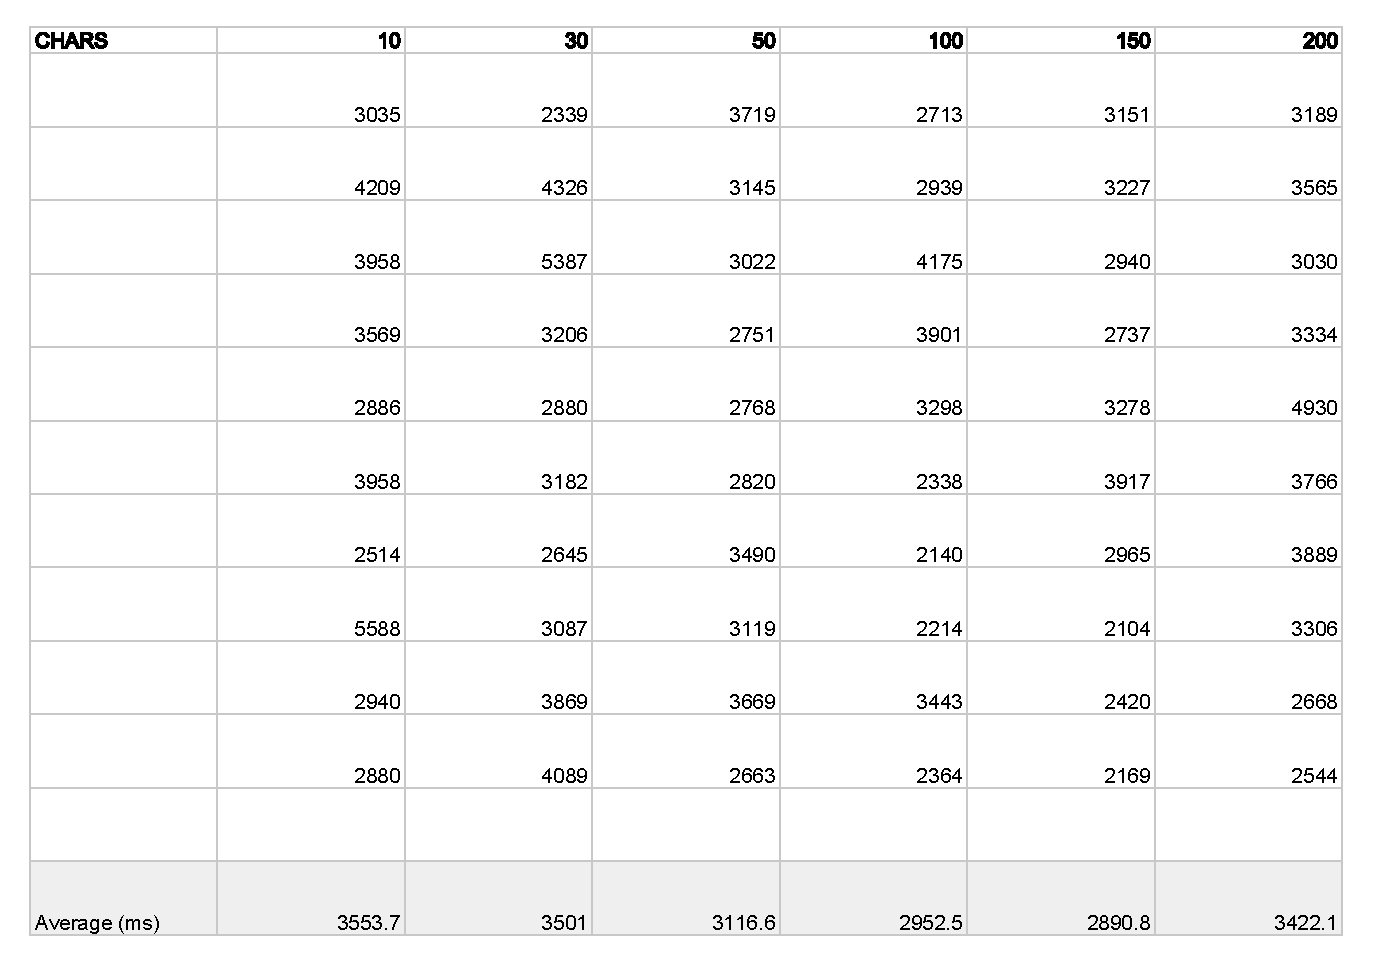
\includegraphics[scale=0.6]{gfx/QR-test.pdf}
	\caption{The results from the QR code test, all times are in ms.}
	\label{fig:QR-code-test}
\end{figure}

\chapter{Usability Test}
\label{usability_test}
\section{Test Invitation}
\begin{figure}[h!]
	\centering
	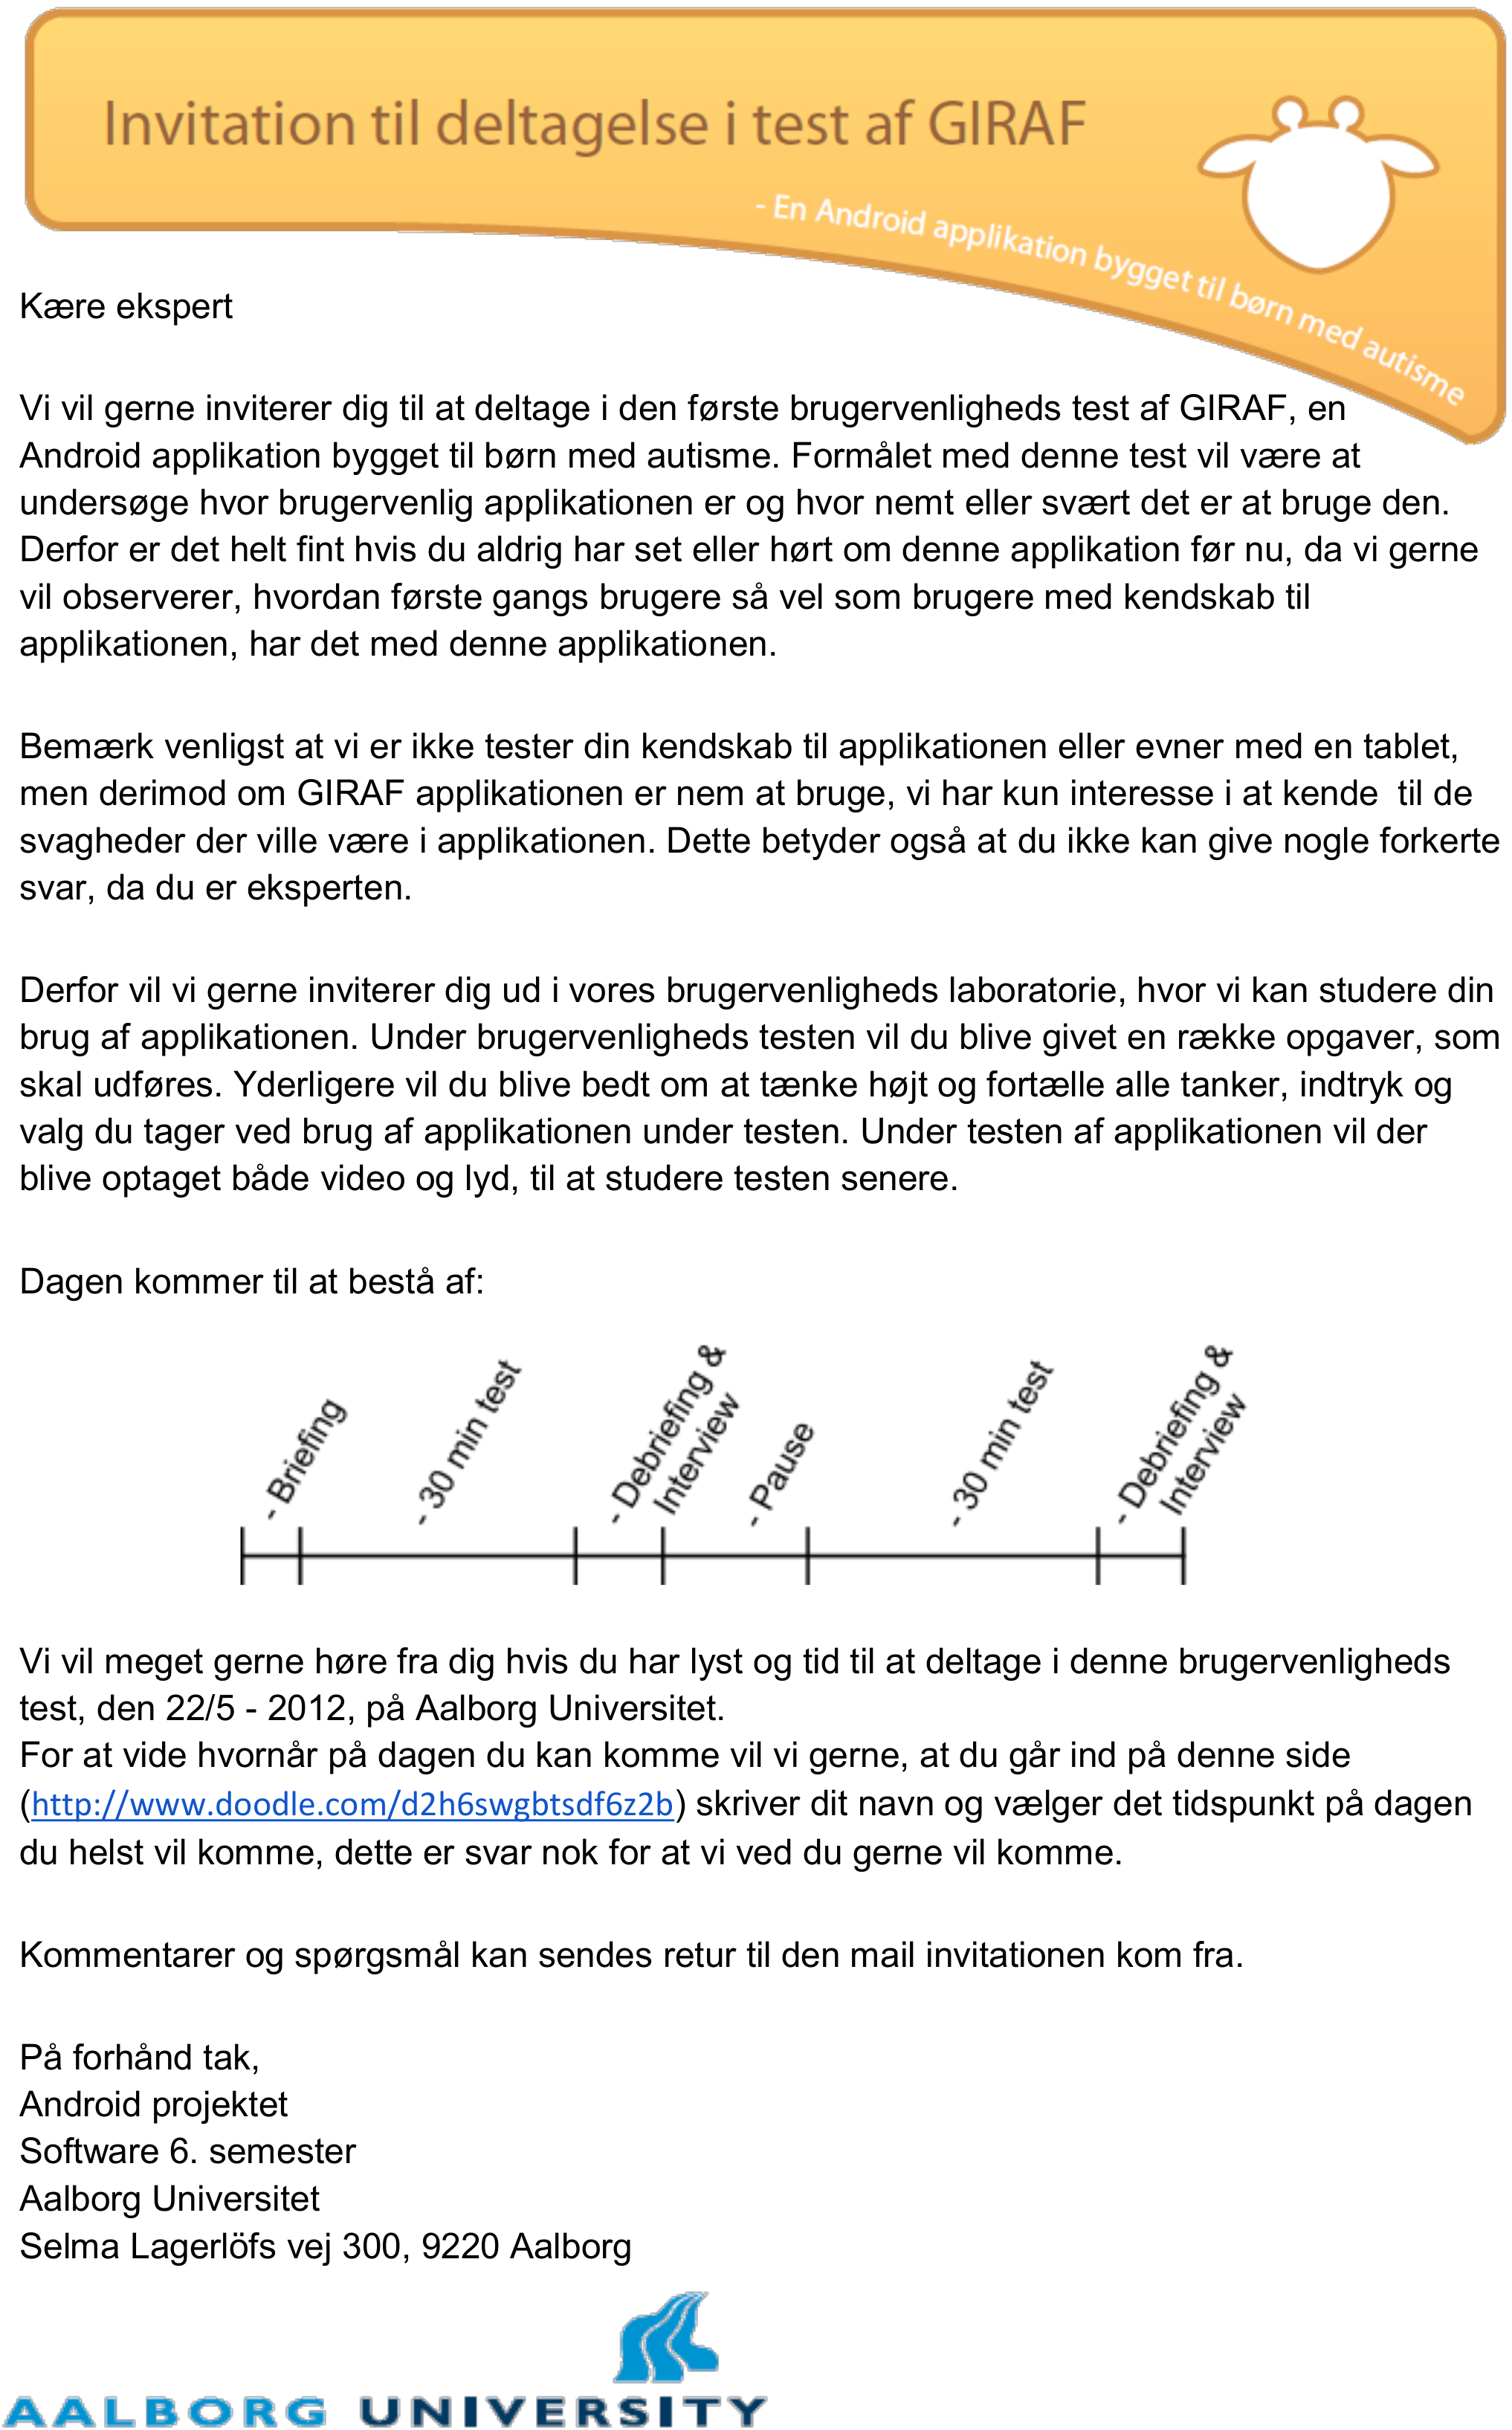
\includegraphics[scale=0.65]{gfx/usabilitytest-invitation.png}
	\caption{Invitation asking for customer participation in usability testing.}
	\label{fig:usability_invitation}
\end{figure}

\section{Test Briefing}
\begin{figure}[h!]
	\centering
	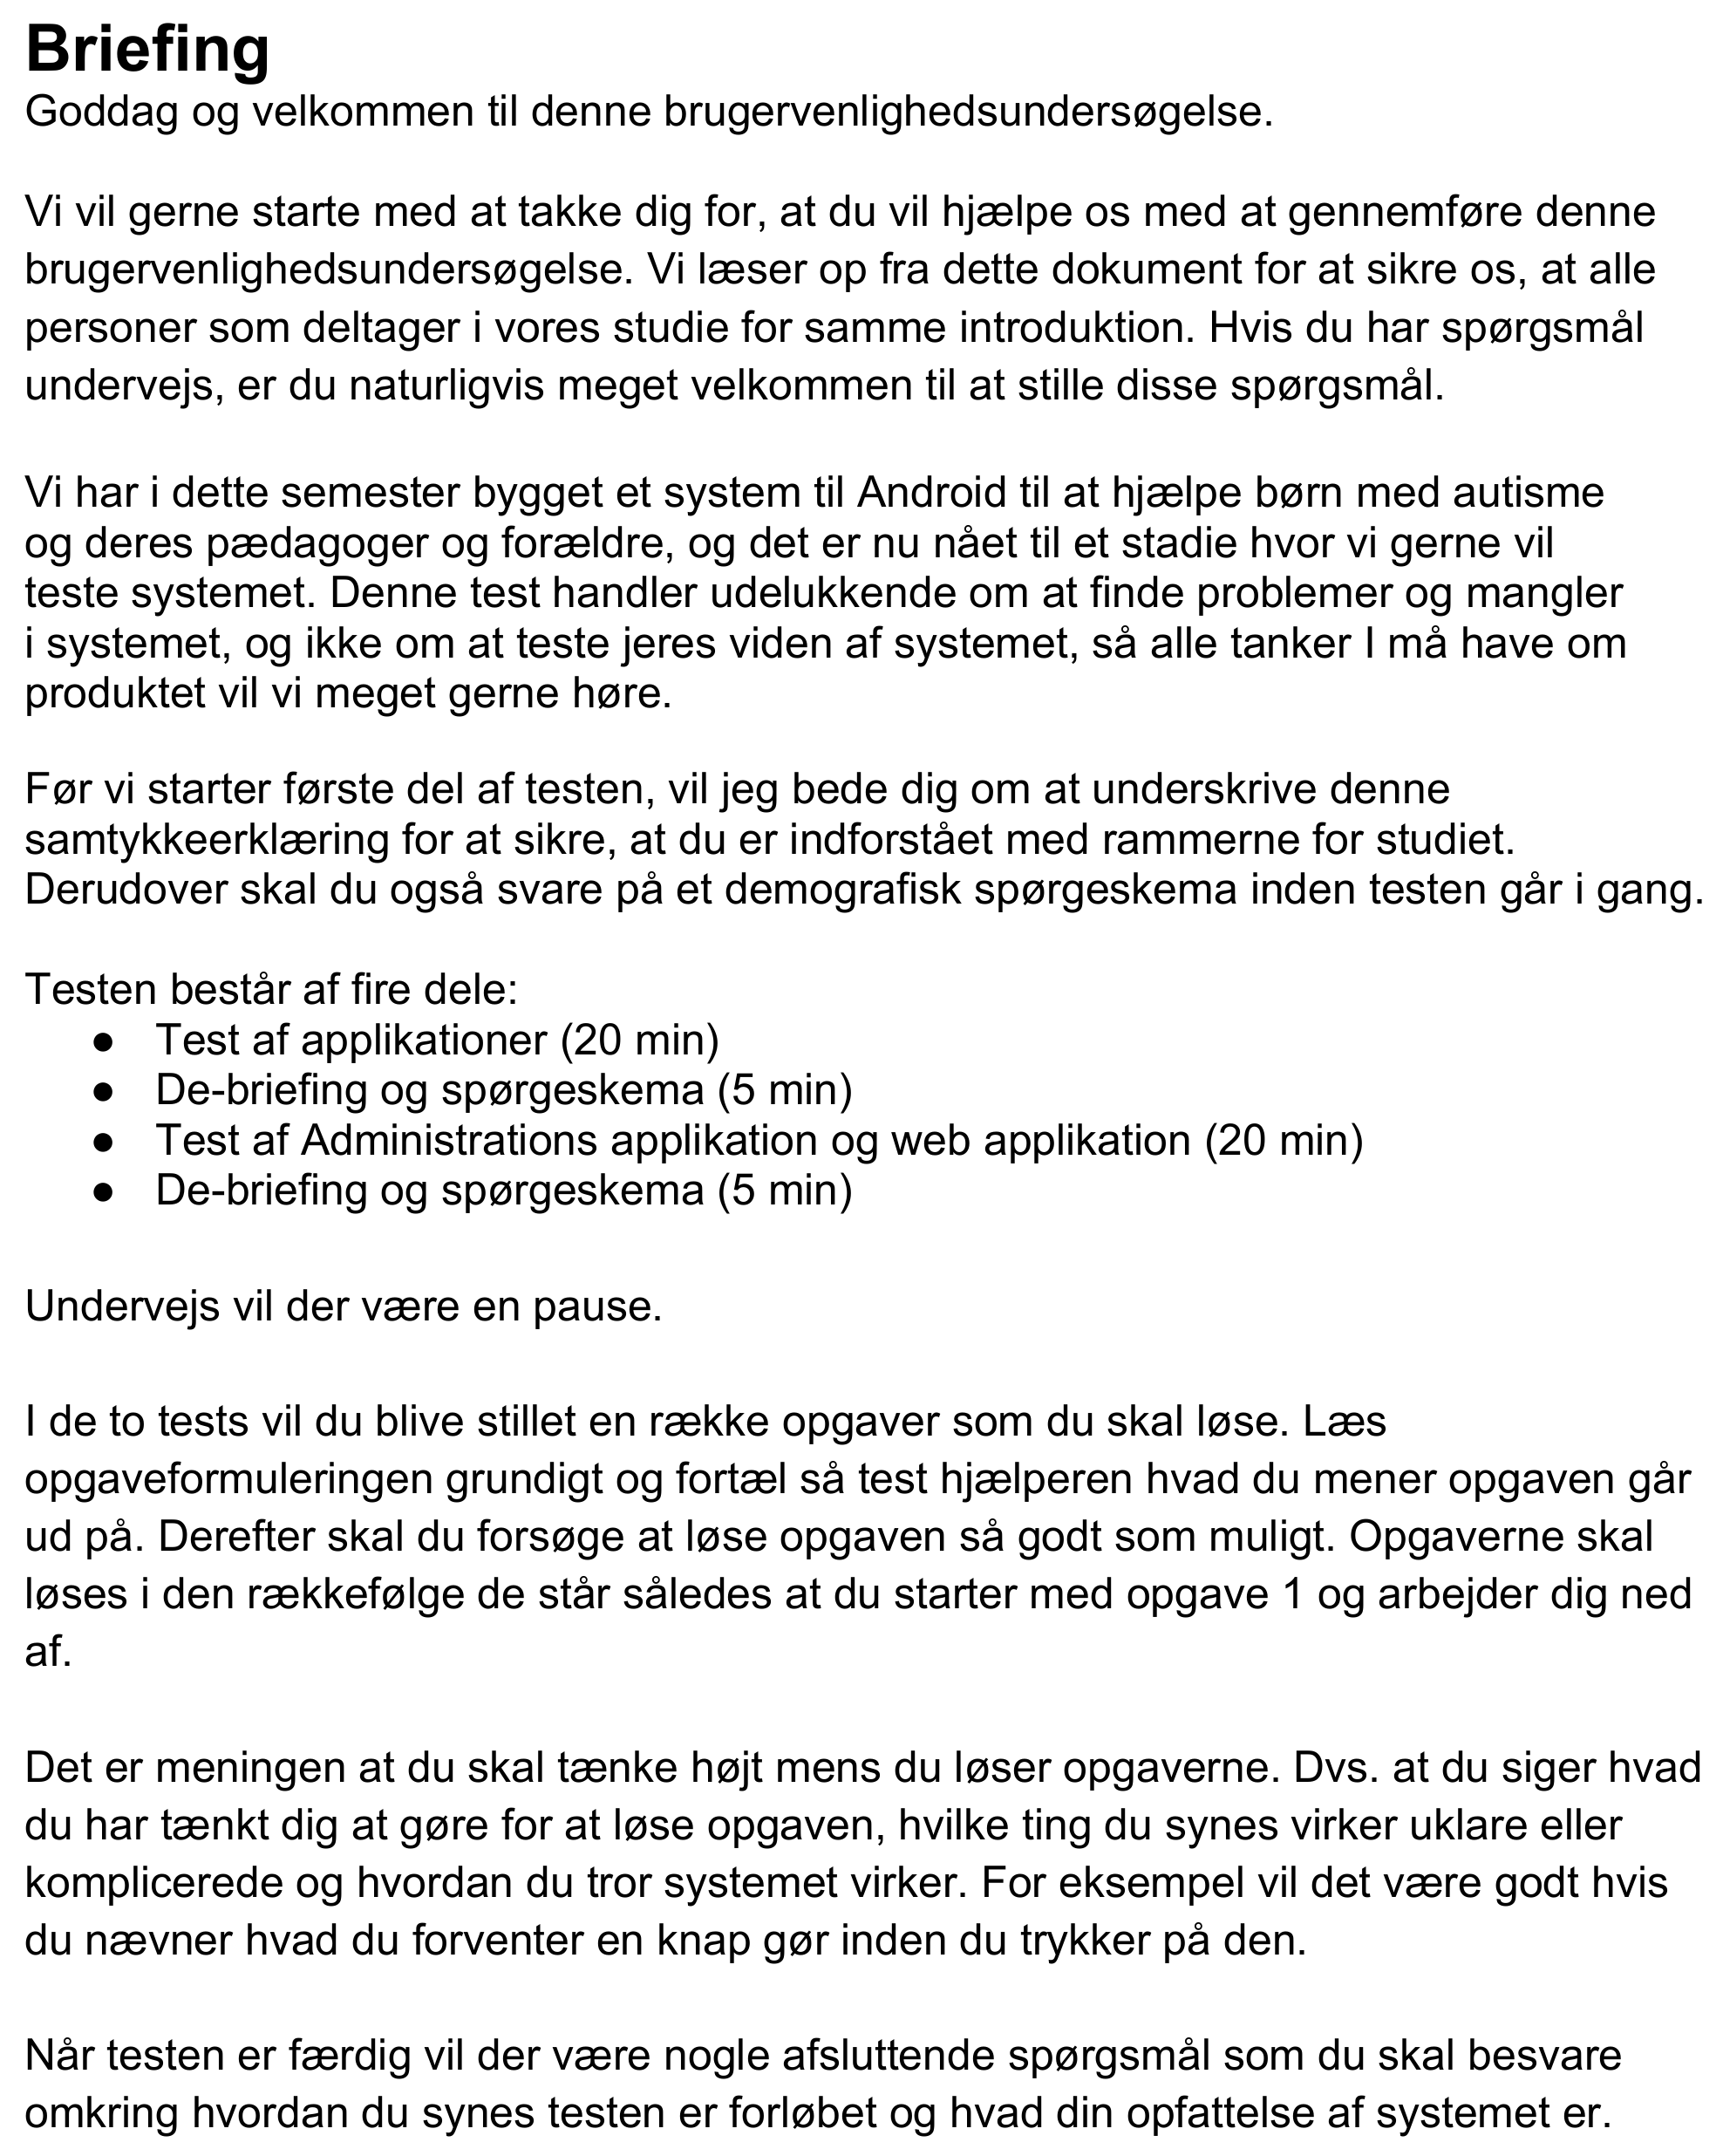
\includegraphics[scale=0.8]{gfx/usability-briefing.png}
	\caption{Briefing given to test subjects prior to testing.}
	\label{fig:usability_briefing}
\end{figure}

\section{Demographic Questionnaire}
\begin{figure}[h!]
	\centering
	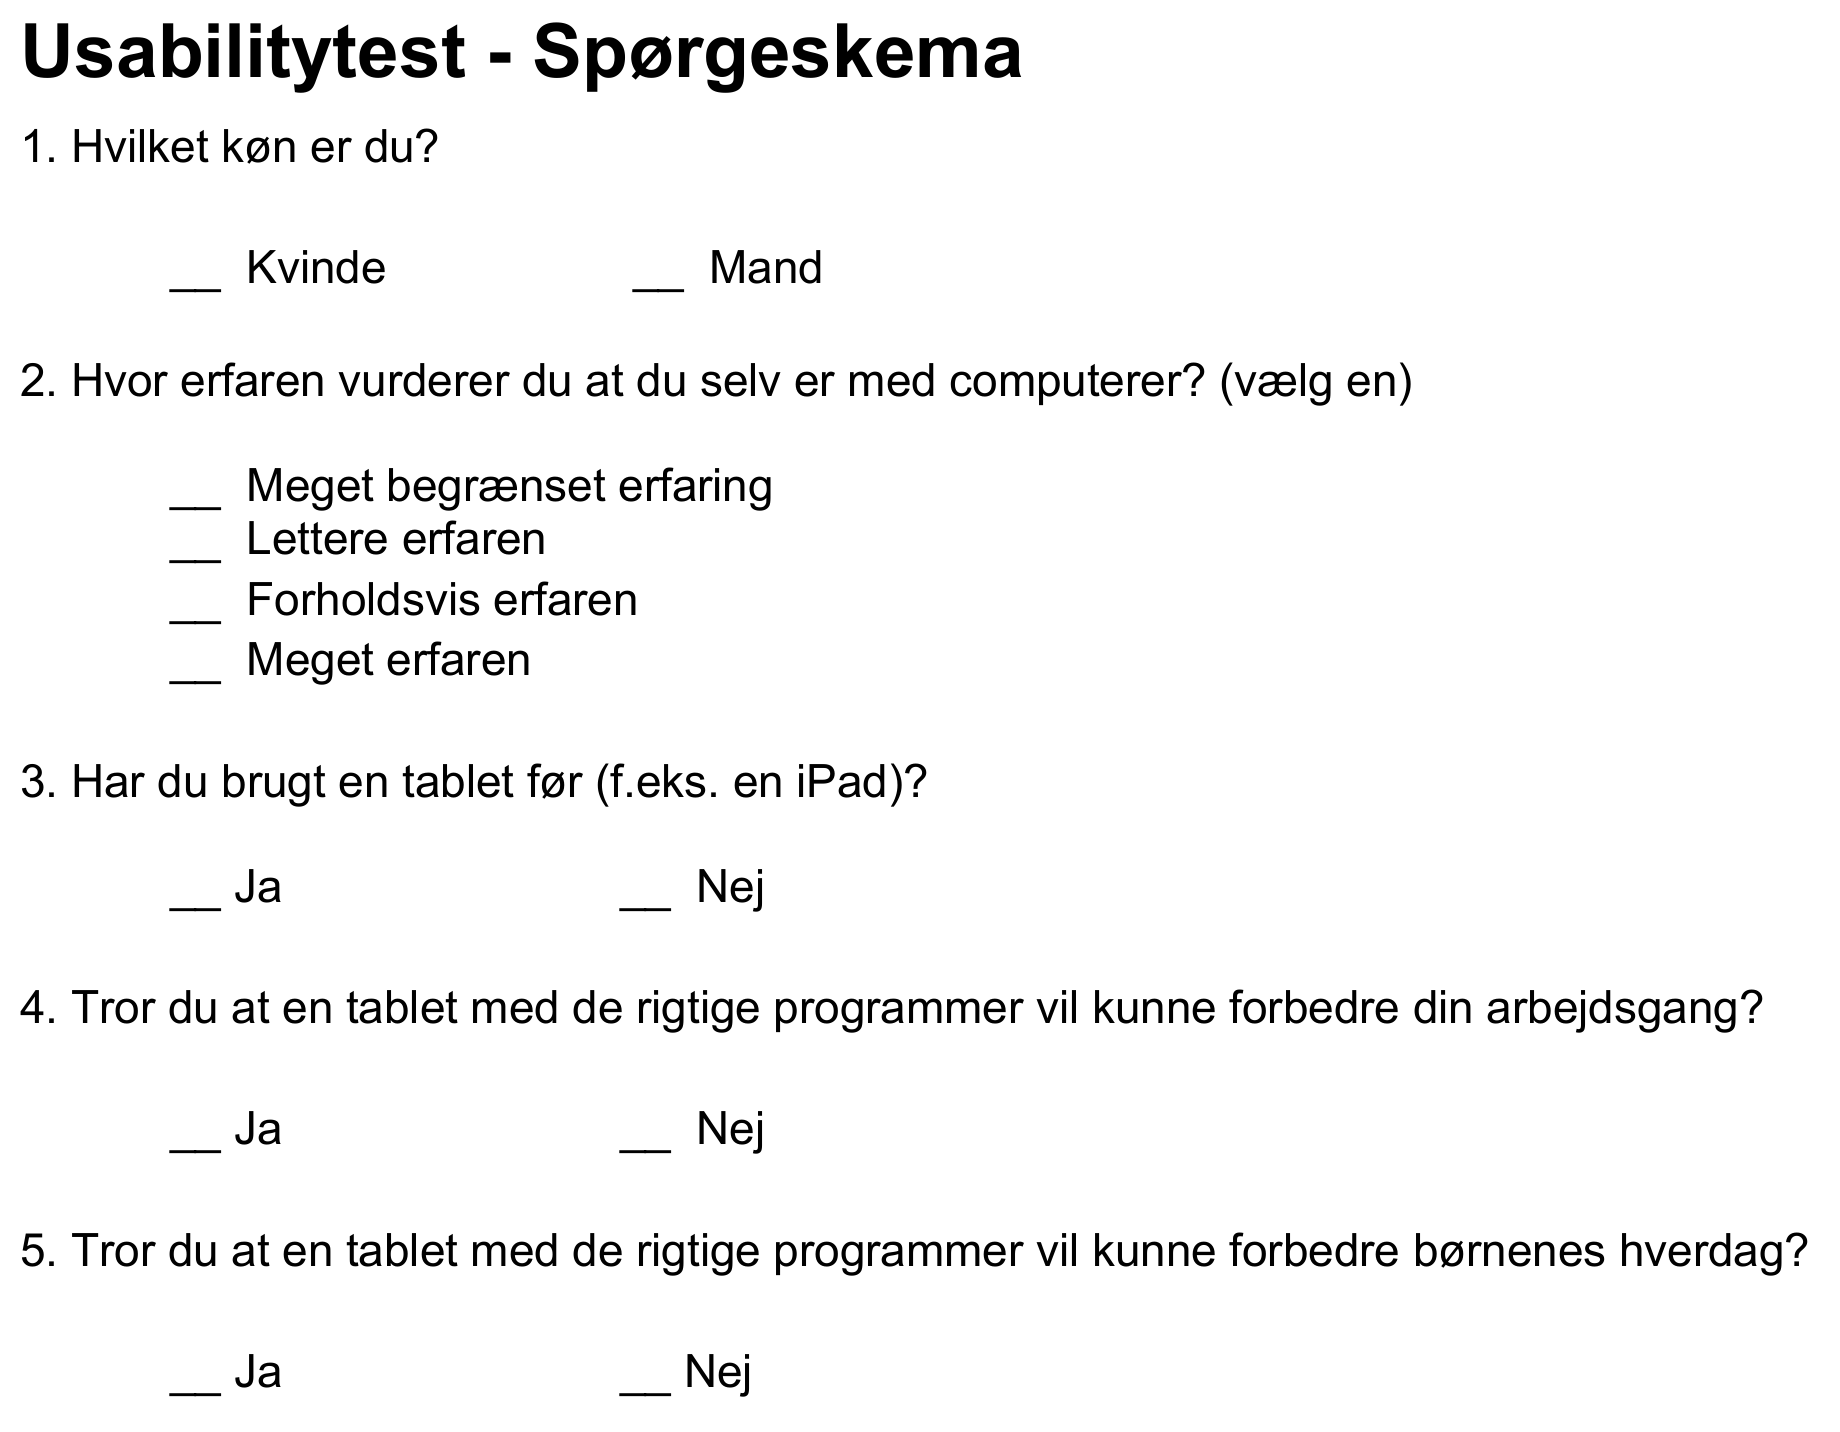
\includegraphics[scale=0.7]{gfx/usability-questionnaire.png}
	\caption{Questionnaire filled out by the test subjects before the test. Afterwards, each subject was asked to rate the difficulty of each application on a five scale rating.}
	\label{fig:usability_questionnaire}
\end{figure}

\chapter{Test Cases}
\label{test_cases}
Overall requirements: \newline
Launcher is installed on a tablet running Android 3.2.x \newline

The tests are grouped based on the class they exist in, with the identifier of each test case being the name of the function tested and the number of the test for that function. \newline

For the second part of the tests of Tools-functions, the following apps must be present in the system as noted for each of them. \newline

WOMBAT (is a GIRAF app):
\begin{itemize}
\item is in the database.
\item is installed on the device.
\item is attached to the current user.
\end{itemize}

PARROT (GIRAF):
\begin{itemize}
\item is in the database.
\item is installed on the device.
\item is \textbf{not} attached to the current user.
\end{itemize}

ViewDB (GIRAF):
\begin{itemize}
\item is \textbf{not} in the database.
\item is installed on the device.
\item is \textbf{not} attached to the current user.
\end{itemize}

Lion (GIRAF):
\begin{itemize}
\item is in the database.
\item is \textbf{not} installed on the device.
\item is \textbf{not} attached to the current user.
\end{itemize}

Leopard (GIRAF):
\begin{itemize}
\item is in the database
\item is \textbf{not} installed on the device.
\item is attached to the current user.
\end{itemize}

Calculator (is an Android app):
\begin{itemize}
\item is in the database.
\item is installed on the device.
\item is attached to the current user.
\end{itemize}

Camera (Android):
\begin{itemize}
\item is in the database.
\item is installed on the device.
\item is \textbf{not} attached to the current user.
\end{itemize}

Gallery (Android):
\begin{itemize}
\item is \textbf{not} in the database.
\item is installed on the device.
\item is \textbf{not} attached to the current user.
\end{itemize}

Internet (Android):
\begin{itemize}
\item is in the database.
\item is \textbf{not} installed on the device.
\item is \textbf{not} attached to the current user.
\end{itemize}

Mail (Android):
\begin{itemize}
\item is in the database
\item is \textbf{not} installed on the device.
\item is attached to the current user.
\end{itemize}

\begin{table}[ht]
\caption{Test cases for the AppAdapter class} % title of Table
\centering  % used for centering table
\begin{tabular}{| p{1.7in} | p{1.7in} | p{1.7in} |}
\hline
Name: & Test: & Pass Criteria: \\ [0.5ex] % inserts table 
%heading
\hline                  % inserts single horizontal line
setAppBackground-001: & Call setAppBackground with the color 0xFFFFFFFF. & The background of the app is the color 0xFFFFFFFF. \\ \hline 
saveAppBackground-001: & Call saveAppBackground with the color 0xFFFFFFFF. & The launcher settings are changed so the color for the given app is 0xFFFFFFFF. \\ [1ex]      % [1ex] adds vertical space
\hline %inserts single line
\end{tabular}
\label{table:appadapter_tests} % is used to refer this table in the text
\end{table}

\begin{table}[ht]
\caption{Test cases for the AppInfo class} % title of Table
\centering  % used for centering table
\begin{tabular}{| p{1.7in} | p{1.7in} | p{1.7in} |}
\hline
Name: & Test: & Pass Criteria: \\ [0.5ex] % inserts table 
%heading
\hline    
setGuardian-001: & Call setGuardian with a non-guardian profile. & The guardian of the AppInfo is null. \\ \hline 
setGuardian-002: & Call setGuardian with a guardian profile. & The guardian of the AppInfo is the guardian used as input. \\ \hline
getShortenedName-001: & Call getShortenedName on an AppInfo with a name of five characters. & The return value is equal to the name of the AppInfo. \\ \hline 
getShortenedName-002: & Call getShortenedName on an AppInfo with a name of six characters. & The return value is equal to the name of the AppInfo. \\ \hline 
getShortenedName-003: & Call getShortenedName on an AppInfo with a name of seven characters. & The returned string consists of six characters with "`..."' concatinated. \\ [1ex] 
\hline %inserts single line
\end{tabular}
\label{table:appinfo_tests} % is used to refer this table in the text
\end{table}

\begin{table}[ht]
\caption{Test cases for the AuthenticationActivity class} % title of Table
\centering  % used for centering table
\begin{tabular}{| p{1.7in} | p{1.7in} | p{1.7in} |}
\hline
Name: & Test: & Pass Criteria: \\ [0.5ex] % inserts table 
%heading
\hline    
changeCamerafeed\newline{}BorderColor-001: & Scan an invalid QR code. & The camera feed border changes to red. \\ \hline 
changeCamerafeed\newline{}BorderColor-002: & Scan a valid QR code. & The camera feed border changes to green. \\ \hline
handleDecode-001: & Scan an invalid QR code. & The camera feed border changes to red and no log-in button and name is shown. \\ \hline 
handleDecode-002: & Scan a valid QR code. & The camera feed border changes to green, a log-in button appears, the name of the user attached to the QR code appears and the device vibrates. \\ [1ex] 
\hline %inserts single line
\end{tabular}
\label{table:authenticationactivity_tests} % is used to refer this table in the text
\end{table}

\begin{table}[ht]
\caption{Test cases for the HomeActivity class} % title of Table
\centering  % used for centering table
\begin{tabular}{| p{1.7in} | p{1.7in} | p{1.7in} |}
\hline
Name: & Test: & Pass Criteria: \\ [0.5ex] % inserts table 
%heading
\hline    
onBackPressed-001: & Press the device back button while on the home screen. & Nothing happens. \\ \hline 
calculateNumOfColumns-001: & The user should have nine apps visible to them. Call calculateNumOfCollumns(). & The returned number is four. \\ \hline
calculateNumOfColumns-002: & The user should have ten apps visible to them. Call calculateNumOfCollumns(). & The returned number is four. \\ \hline 
calculateNumOfColumns-003: & The user should have thirteen apps visible to them. Call calculateNumOfCollumns(). & The returned number is five. \\ \hline 
appBgColor-001: & A color for a given app already exists in the settings. Call appBgColor(). & The color returned matches the one from the settings. \\ \hline 
saveNewBgColor-001: & Call saveNewBgColor() with a real color and the ID of an app in the database. & This color has been saved in the settings. \\ \hline 
saveNewBgColor-002: & Call saveNewBgColor() with null as a color and the ID of an app in the database. & The settings are not changed. \\ \hline 
saveNewBgColor-003: & Call saveNewBgColor() with a real color and null as the ID. & The settings are not changed. \\ [1ex] 
\hline %inserts single line
\end{tabular}
\label{table:homeactivity_tests} % is used to refer this table in the text
\end{table}

\begin{table}[ht]
\caption{Test cases for the ProfileSelectActivity class} % title of Table
\centering  % used for centering table
\begin{tabular}{| p{1.7in} | p{1.7in} | p{1.7in} |}
\hline
Name: & Test: & Pass Criteria: \\ [0.5ex] % inserts table 
%heading
\hline                  % inserts single horizontal line
loadProfiles-001: & Call loadProfiles() for a guardian with children attached and different departments that also have children attached. & The returned list of children contains all children attached to the given guardian and the children attached to the departments of the guardian, but no duplicates. \\ [1ex]  
\hline %inserts single line
\end{tabular}
\label{table:profileselectactivity_tests} % is used to refer this table in the text
\end{table}

\begin{table}[ht]
\caption{Test cases for the Tools class, part one} % title of Table
\centering  % used for centering table
\begin{tabular}{| p{1.7in} | p{1.7in} | p{1.7in} |}
\hline
Name: & Test: & Pass Criteria: \\ [0.5ex] % inserts table 
%heading
\hline    
saveLogInData-001: & Login as an valid guardian. & The correct ID and timestamp is saved in shared preferences. \\ \hline 
findCurrentUser-001: & Call findCurrentUser(). & The currently logged in profile is returned. \\ \hline
findCurrentUserID-001: & Call findCurrentUserID(). & The currently correct profile ID is returned. \\ \hline 
clearAuthData-001: & Call clearAuthData(). & The ID is set to -1 and time to 1 in the shared preferences. \\ \hline 
sessionExpired-001: & Let the session to expire after 1 minute. \newline Log in as a valid guardian. Turn off device. Wait one minuted. Turn on device. & The guardian is logged out. \\ [1ex] 
\hline %inserts single line
\end{tabular}
\label{table:tools_tests1} % is used to refer this table in the text
\end{table}

\begin{table}[ht]
\caption{Test cases for the Tools class, part two (where the app requirements are enforced)} % title of Table
\centering  % used for centering table
\begin{tabular}{| p{1.7in} | p{1.7in} | p{1.7in} |}
\hline
Name: & Test: & Pass Criteria: \\ [0.5ex] % inserts table 
%heading
\hline    
getVisibleGirafApps-001: & Call getVisibleGirafApps() for the current user. & Only Wombat is returned. \\ \hline 
getVisibleAndroidApps-001: & Call getVisibleAndroidApps() for the current user. & Only Calculator is returned. \\ \hline
getVisibleApps-001: & Call getVisibleApps() for the current user. & Only Wombat and Calculator are returned. \\ \hline 
getHiddenGirafApps-001: & Call getHiddenGirafApps() for the current user. & Only Parrot is returned. \\ \hline 
getHiddenAndroidApps-001: & Call getHiddenAndroidApps() for the current user. & Only Camera is returned. \\ \hline 
getHiddenApps-001: & Call getHiddenApps() for the current user. & Only Parrot, ViewDB, Lion, Camera, Gallery and Internet are returned. \\ \hline 
getAvaliableGirafApps-001: & Call getAvaliableGirafApps() for the current user. & Only Wombat and Parrot are returned. \\ \hline 
getAvaliableAndroidApps-001: & Call getAvaliableAndroidApps() for the current user. & Only Calculator and Camera is returned. \\ \hline 
getAvaliableApps-001: & Call getAvaliableApps() for the current user. & Only Wombat, Parrot, Calculator and Camera is returned. \\ \hline 
getDeviceGirafApps-001: & Call getDeviceGirafApps() for the current user. & Verify that Wombat, Parrot and ViewDB is shown. \\ \hline 
getDeviceAndroidApps-001: & Call getDeviceAndroidApps() for the current user. & Only Calculator, Camera and Gallery is returned. \\ \hline 
getDeviceApps-001: & Call getDeviceApps() for the current user. & Only Wombat, Parrot, ViewDB, Calculator, Camera and Gallery is returned. \\ \hline 
subtractAppsList-001: & Call subtractAppsList with a[wombat,Calculator] and b[Calculator]. & Only Wombat is returned. \\ [1ex] 
\hline %inserts single line
\end{tabular}
\label{table:tools_tests2} % is used to refer this table in the text
\end{table}

\begin{table}[ht]
\centering  % used for centering table
\begin{tabular}{| p{1.7in} | p{1.7in} | p{1.7in} |}
\hline  
packageRegistered-001: & Call packageRegistered() with Wombat. & True is returned. \\ \hline 
packageRegistered-002: & Call packageRegistered() with ViewDB. & False is returned. \\ \hline 
insertAppInDB-001: & Call insertAppInDB() with ViewDB. & ViewDB is now in the database. \\ \hline 
attachLauncher-001: & A relation between the launcher and given user does not currently exist. Call attachLauncher() with the given user. & A relation between the launcher and user now exists in the database. \\ \hline 
appsContain\_{}RI-001: & Call appsContain\_{}RI with list of apps installed on the device as ResolveInfo's and Parrot. & True is returned. \\ \hline 
appsContain\_{}RI-002: & Call appsContain\_{}RI with list of apps installed on the device as ResolveInfo's and Lion. & False is returned. \\ \hline 
appsContain\_{}A-001: & Call appsContain\_{}A with a list of apps in the database and Wombat. & True is returned. \\ \hline 
appsContain\_{}A-002: & Call appsContain\_{}A with a list of apps in the database and ViewDB. & False is returned. \\ [1ex] 
\hline %inserts single line
\end{tabular}
\end{table} % Appendix

\cleardoublepage% Bibliography

\label{app:bibliography} % Reference the bibliography elsewhere with \autoref{app:bibliography}

\manualmark
\markboth{\spacedlowsmallcaps{\bibname}}{\spacedlowsmallcaps{\bibname}} 
\refstepcounter{dummy}

\addtocontents{toc}{\protect\vspace{\beforebibskip}} % Place the bibliography slightly below the rest of the document content in the table of contents
\addcontentsline{toc}{chapter}{\tocEntry{\bibname}}

\bibliographystyle{plainnat}

\bibliography{Bibliography} % Bibliography

%----------------------------------------------------------------------------------------

\end{document}
